%%%%%%%%%%%%%%%%%%%%%%%%%%%%%%%%%%%%%%%%%%%%%%%%%%%%%%%%%%%%%%%%%%%%%%
% How to use writeLaTeX: 
%
% You edit the source code here on the left, and the preview on the
% right shows you the result within a few seconds.
%
% Bookmark this page and share the URL with your co-authors. They can
% edit at the same time!
%
% You can upload figures, bibliographies, custom classes and
% styles using the files menu.
%
%%%%%%%%%%%%%%%%%%%%%%%%%%%%%%%%%%%%%%%%%%%%%%%%%%%%%%%%%%%%%%%%%%%%%%

\documentclass[12pt]{article}

\usepackage{sbc-template}

\usepackage{graphicx,url}

%\usepackage[brazil]{babel}   
\usepackage[utf8]{inputenc}  

     
\sloppy

\title{Native Language Classification\\ with Minimal Resource}

\author{Rafael Melo\inst{1}, Tiago Barbosa de Lima\inst{1}}


\address{Departamento de Computação -- Universidade Federal Rural de Pernambuco
  (UFRPE)\\
  Recife, -- PE -- Brazil
  \email{\{tiago.blima,rafael.melo\}@ufrpe.br}
}

\begin{document}

\maketitle

\begin{abstract}
   There are around 45 million native people in Latin America; 190 thousand of them live in Brazil. Despite that, there is a lake of resource of their language. Moreover, the currents translation platform like google and bing translator does not provide an automatic identification for them. Therefore, this paper gives a step toward the development of a method to automatic classify Brazilian native language with the minimal resource available.
\end{abstract}


\section{Introduction}\label{sec:introduction}

According to the International Labour Organisation (ILO) 169 agreement over native people; it is possible to identify a group of indigenous using some aspects.
The considered features are the territory, identity recognition, common origin, culture and language \cite{povos_indigenas}.
Furthermore, according to \cite{povos_indigenas}, there are 45 million native people only in Latin American.
It shows the importance of the study of their native languages, and the use of computational resources to make it accessible.

Besides, computers have taken a prominent part of our lives, mainly in the day to day tasks \cite{matthews2016introduction}. 
Moreover, most of the human communication uses natural language\cite{matthews2016introduction}. 
It would be of great importance for the development of a process to make the human language able to be understood by the computers~\cite{matthews2016introduction}.
One example of the use of natural language processing in our day to day is google translator~\cite{google}.

One of the resources provided by google translator is classifying a given text by the language and therefore is a good example of the purpose of this paper. 
It achieved using today's wide used method known as the natural language process.
It comes from the result of the use of artificial intelligence and linguistic\cite{10.1136/amiajnl-2011-000464}.
Besides, it seeks to fill this gap between computer and human communication.
 Also, it has suffered a great explosion of works focusing on several languages groups\cite{peters2002evaluation}.

Therefore, considering the great importance of the native languages and its identification for a computational system.
We use the tools of the natural language processing and information retrieval to identify and classify 26 Brazilian native languages and the Portuguese.

\section{Brazilian Native Languages} \label{sec:firstpage}
  
  Although, according to \cite{povos_indigenas} there are 900 thousand native people only in Brazil.
  The lack of resources is one of the biggest concerns in the development of a natural language processing method to native languages.
  Once the languages like the ones from Tupi have an oral tradition;
  there are only a few texts available for computational analyses.
  Besides, some of the languages native of Latin American, have a poly-synthetic nature.
  It means that one single word can represent a whole order, and the Tupi is one of them \cite{lemos1956tupi}.
  This same issue was faced on \cite{DBLP:journals/corr/abs-1804-06024} study.
  The discovered technique to handle this difficulty was to divide the words in the smallest morphological component providing a more extended and varied vocabulary.


\section{Stemming}\label{sec:stemming}

The process of stemming is to reduce a word to its canonical form \cite{Goldsmith:2000:ALS:648263.753378}.
It helps us to control a database of a large data set of documents in the case of an identification
system~\cite{Goldsmith:2000:ALS:648263.753378}.
Based on that, we build the automatic stem proposed by~\cite{Goldsmith:2000:ALS:648263.753378}.
It considers the coherence of several possible suffixes.
The coherence is calculated considering the last seven or fewer letters of a word using the equation (1).

\begin{equation}
    freq(l_1,l_2,..,l_n)log\frac{freq(l_1,l_2,..,l_n)}{freq(l_1)freq(l_2)...freq(l_n)}
\end{equation}
we removed the 300 most frequent words as proposed in the original approach.
After, we select a stem generated by a suffix if there are at least two stems related to it.
We also established a threshold of 5 stems for each used suffix.


\section{Multi-Language Classification}\label{sec:multi-language-classification}

\subsection{Related Works}
   The techniques of multi-language classification have been developed since 1967 \cite{cabral_2015}. Many techniques were used so far; some of them are based on text categorisation using the kernel-based on IDF of n-grams. We can also quote the ones based on the text frequency of specific terms \cite{cabral_2015}.  
   The most well-known example of term frequency based classifier is the TextCat software based on paper \cite{cavnar1994n}. The method developed consists of the generation a profile based on the counts of n-grams. Then, the documents are classified by the similarity between the n-grams of the trained documents and the new document that must be classified.
\subsection{Used Method}
    Despite the techniques quoted, we used a simpler method that consisted exclusively in the analyses of the most frequent words in each language.
    Our classification process consisted of the selection of the 100 most frequent words of each language both in training and test set. It was made after we use the automatic stem explained in the last section. 
    Then, we verify if the word in the list of most frequent words in the test set is also in the training set.  
  


    
\section{Results}\label{sec:results}


The experiment consisted of separating the data in training and test sets. The training sets were the first four books of the New Testament from the bible available at \cite{angelo}. 
Hence, we checked if each 100 most frequent test was also present in the training set. After, we selected the language in training set with the biggest number of common top-ranked words. It is important to note that the order of the ranking was not taken into consideration in the experiment. 
We were able to predict all languages correctly, but with different match percentage outcomes. The result found is exposed in figure 2.


\begin{figure}[h!]
\centering
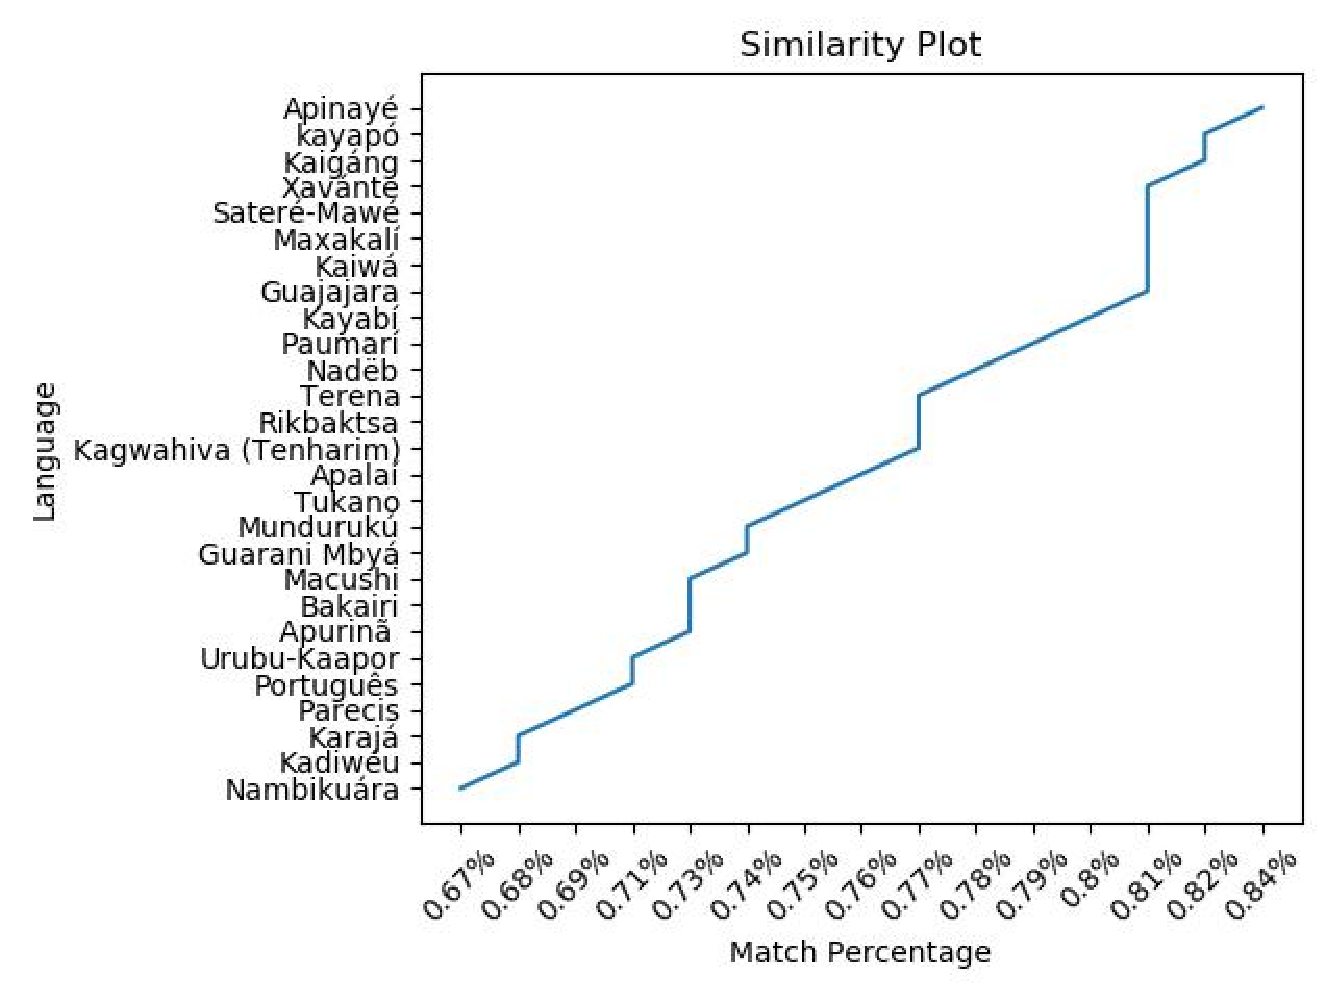
\includegraphics[width=.6\textwidth]{images/fig1.pdf}
\caption{The figure shows the percentage of match of the 100 top rank words of training and test.}
\label{fig:Fig1}
\end{figure}


\subsection{Threshold}\label{subsec:threshold}

Another approach was to verify the behaviour of our method in different train sets. We increased the size of the train set systematically inserting one book each iteration from starting with one book and ending with four. The result found in figure 2 shows the relation between the mean of the percentage of match and the performance.

\begin{figure}[h!]
\centering
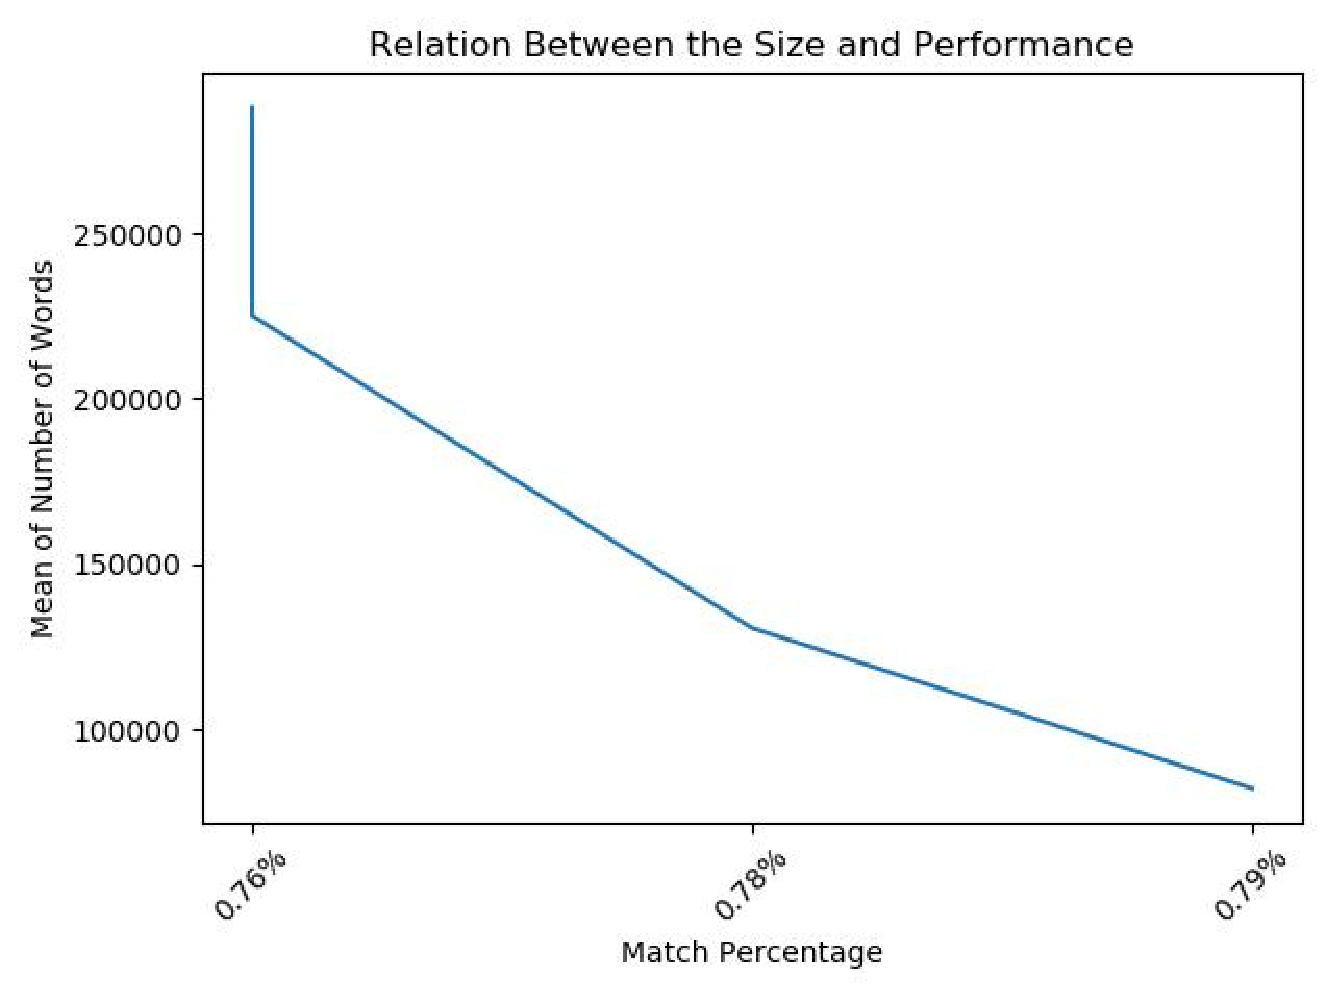
\includegraphics[width=.5\textwidth]{images/fig2.pdf}
\caption{The figure shows the percentage of match through different threshold tests.}
\label{fig:Fig1}
\end{figure}

\begin{center}
\begin{tabular}{ ||c c c c|| }
\hline
Mean Number of Words & Mean Word Match & Match Standard Deviation & Hits\\ [0.5ex]
\hline\hline
82125 & 0.79\% & 0.06 & 27\\
130567.85 & 0.78\% & 0.06 & 27\\
225235.70 & 0.76\% & 0.05 & 27\\
288065.74 & 0.76\% & 0.05 & 27\\
\hline
\end{tabular}
\end{center}

\section{Acknowledgement}
    The experiments were possible thanks to the efforts made to translate the 26 New Testament of the bible native languages and the availability of them at~\cite{angelo}.
    
\section{Conclusion}\label{sec:conclusion}


This work introduces a method to identify Brazilian native languages with successful results, despite the minimal resources available.
Consequently, costly methods such as the ones that use neural networks or need a large data set size could be easily replaced by our method.
It also was an important step in the direction of turning  Brazilian languages more accessible. 


\bibliographystyle{sbc}
\bibliography{sbc-template}

\end{document}
